\chapter{Implementácia systému}

Z kapitoly \ref{vyber} vyšlo že Linode je najlepšia volba pre virtuálne prostredie na nasadaenie mojho malého e-shopu. Vytvrenie prostredie bolo jednoduché ako je možné vidiet na obrázkoch \ref{img:one} a \ref{img:two}.

\begin{figure}[ht!]
  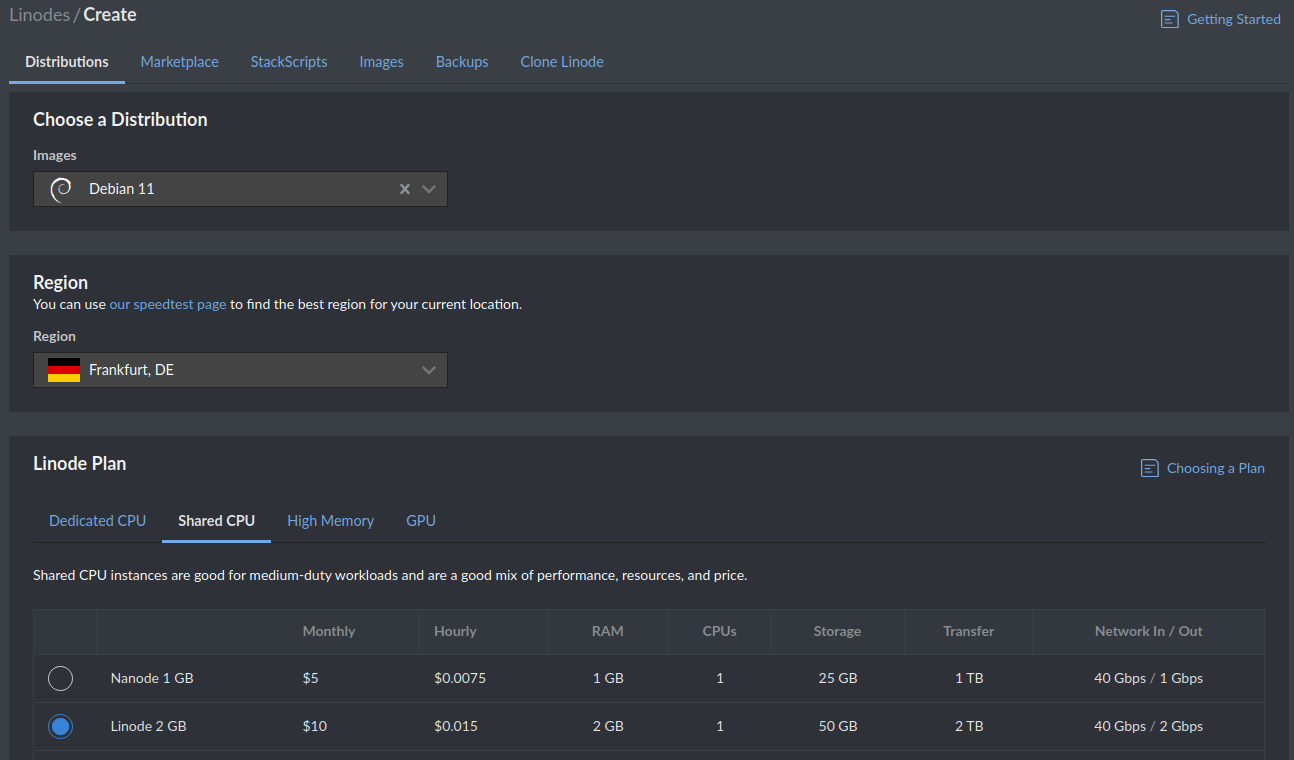
\includegraphics[width=\linewidth]{images/1.png}
  \caption{Prvá časť vytvorenia virtualného prostredia}
  \label{img:one}
\end{figure}

\begin{figure}[ht!]
  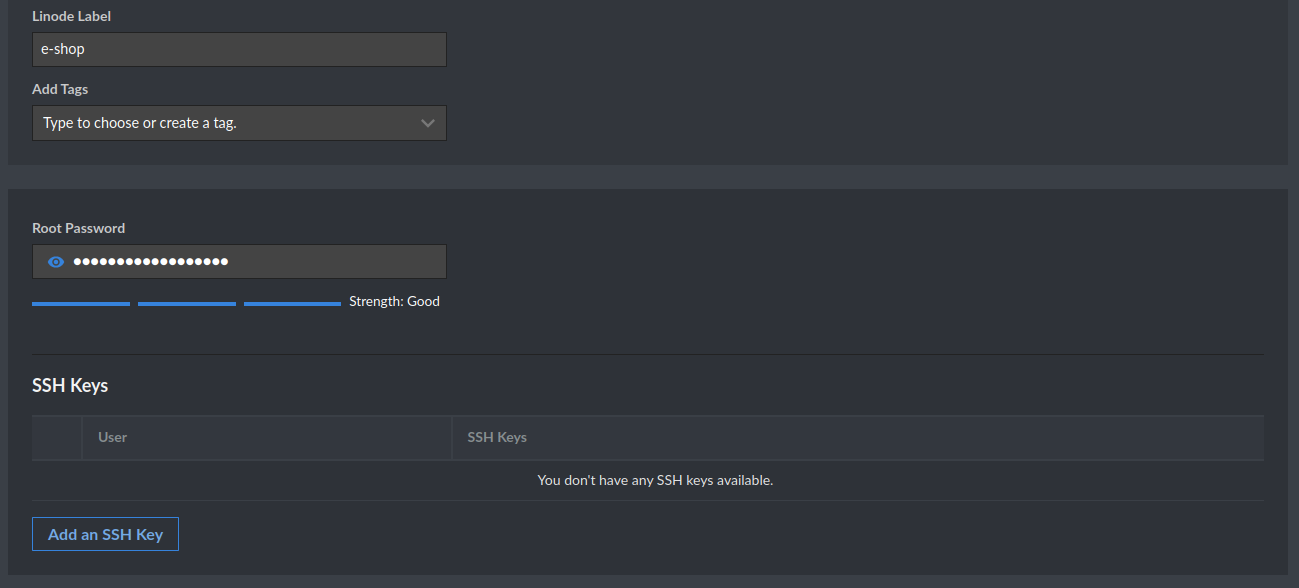
\includegraphics[width=\linewidth]{images/2.png}
  \caption{Druhá časť vytvorenia virtualného prostredia}
  \label{img:two}
\end{figure}

\noindent Uživatelské rozhranie ovládacieho panelu pre linode je velmi intuitívne a prehľadné ako je zase možné vidieť na obrázkoch \ref{img:three} a \ref{img:four}.

\begin{figure}[ht!]
  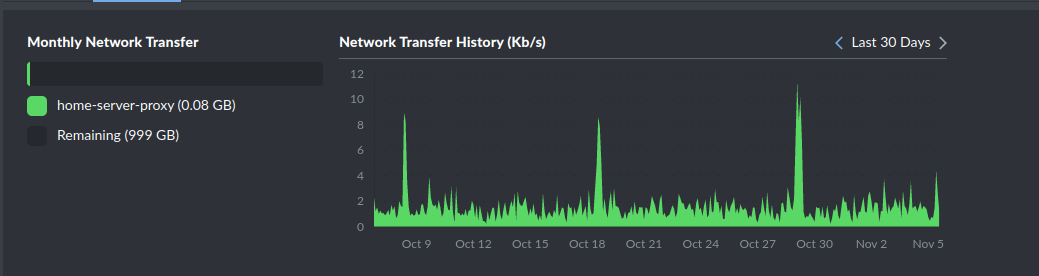
\includegraphics[width=\linewidth]{images/3.png}
  \caption{Prehľad sieťového provozu}
  \label{img:three}
\end{figure}

\begin{figure}[ht!]
  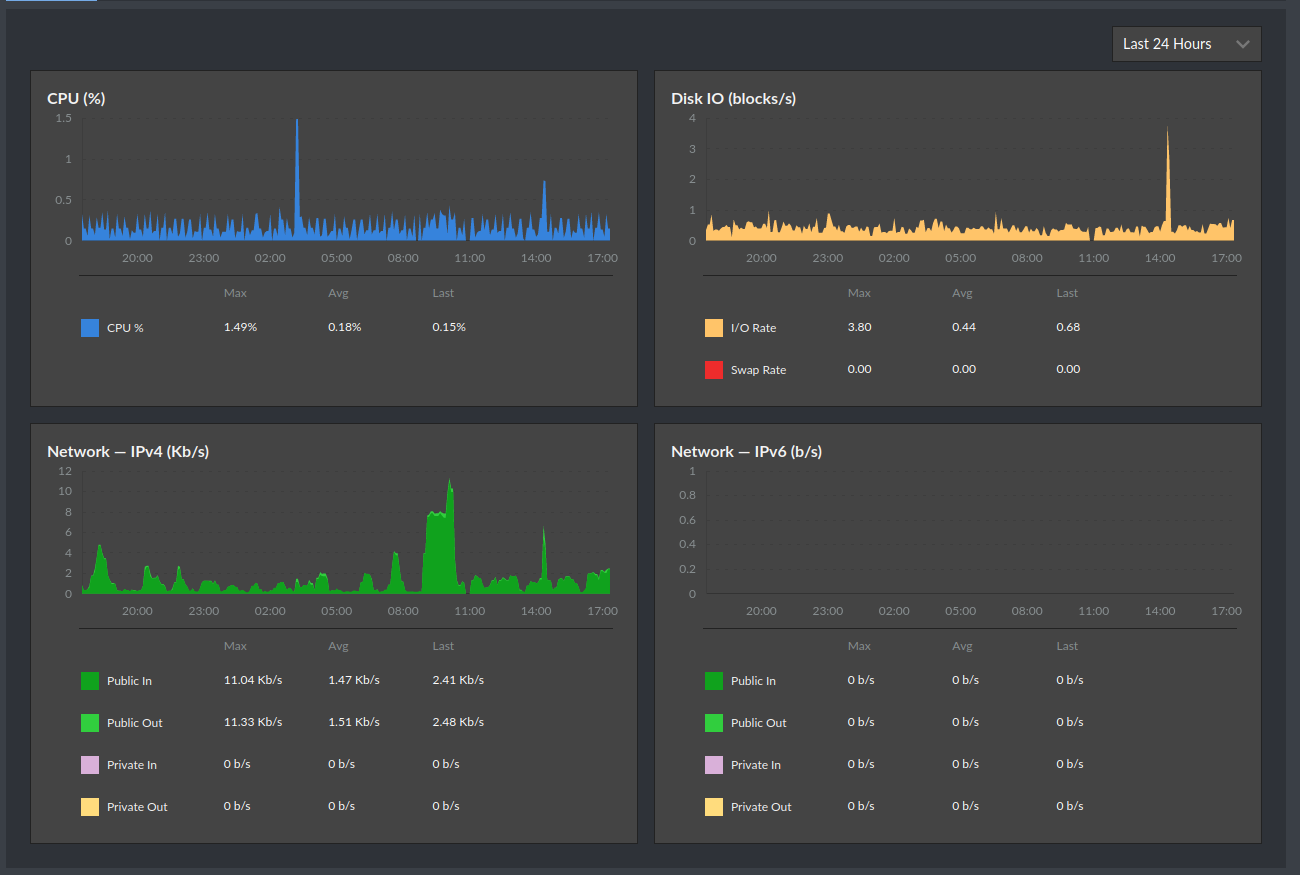
\includegraphics[width=\linewidth]{images/4.png}
  \caption{Prehľad systému}
  \label{img:four}
\end{figure}

\noindent Ako prvé som nastavil potrebné bezpečnostné opatrenia:
\begin{itemize}
  \item Nastavenie firewallu pomocou iptables,
  \item Nastavenie prihlásenia iba cez ssh klúč,
  \item Nainštalovať všetky potrebné nástroje a aplikácie na spustenie mojej vyvinutej aplikácie,
  \item Nastavenie automatický update balíčkov z verziami ktoré obsahujú bezpečnostné vylepšenia.
\end{itemize}

Další krok bude zakúpenie doménového mena pomocou stránky \cite{domain}. Aby bolo možné doménu využívať doménu na internete, bude potreba vytvorit globálny preklad domény na IP adresu môjho serveru, na toto využijem Google Cloud DNS \cite{dns}. Keďže bude stránka podporvať protokol HTTPS, potrebuje aj certifikát. Certifikát budem kupovať na moje doménove meno cez ssls.com \cite{cert}. Predpokladná suma pre doménu, DNS preklad a certifikát je 9\,\texteuro~na mesiac. V cene pre DNS preklad je 10 miliónov prekladov za mesiac čo by na začiatku predaja mojich služieb bude stačiť. cene Platobná braná z ktorú ingergrujem do mojej stránky bude paypal. Pre frontend aplikácie použuijem tému Now UI Kit \cite{vue_kit}.
